\chapter{Related Work}
%Add some context information and introduction before delving into the related work.
%There are many possibilies in the world of web-education, some of the tools we will look at have features such as automatic feedback, static code analysis, adaptive difficulty, automated exercise generation, dynamic code analysis, marking code according to style, correctness, etc...

%It is not uncommon for universities to have their own web infrastructure allowing for submission of exercises, class modules, etc..

%We look at how these related works have approached some of the components of a web education system, such as generating exercises, adaptive difficulty, etc...

%We select these related works because they all have at least one feature that we are interested in implementing into jSCAPE.

Web-based/Computer based education and adaptive web-based assessment systems are a ``hot" research area, and as a result, numerous tools, environments and infrastructures have emerged over the years. There are common features to all, however some distinguish themselves by having not so common features.
Automated exercise generation in these tools is usually non-existent or very limited. Moreover, the tools are more focused on assessing students rather than self-assessment, i.e. students take tests which count towards their final grade on these systems.\newline

There are many components involved in this project, two of the more important ones are adaptive difficulty and automated generation of exercises, so there are many tools which exist which do one or the other, very rarely both.\newline

In this section we look at related software and evaluate them with respect to the objectives listed at the beginning of the development of jSCAPE.

\section{Environment for Learning to Program}
Environment for Learning to Program (ELP) is an interactive web based environment for teaching programming to first year Information Technology students at Queensland University of Technology (QUT).

\section{CourseMarker}
CourseMarker is a re-design of Ceilidh, a computer based assessment system used at the University of Nottingham for 13 years. Ceilidh was quite a complete system, providing coursework, the management of modules and the presentation of module content.

\section{AEGIS}
The Automatic Exercise Generator with Tagged Documents based on the Intelligence of Students (AEGIS)

\section{Programming Adaptive Testing}
PAT\cite{PAT} is a web-based adaptive testing system, developed in ActionScript/Flash, for assessing students' programming knowledge in Greek high schools. \newline

The assessment is carried out by presenting students with 30 questions from various chapters of the introductory programming course. Some of the questions supported by the PAT system are true/false questions, multiple choice questions, gap filling in a piece of code, questions involving diagrams and questions where one has to determine the behaviour of a piece of code.\newline

In PAT, questions are classified into different difficulty categories. Category A is for easy questions, category B is for intermediate questions and category C is for difficult questions. PAT seeks to adapt the difficulty of the questions to the student's ability, by choosing questions of the appropriate difficulty category.

\begin{figure}[H]
\centering
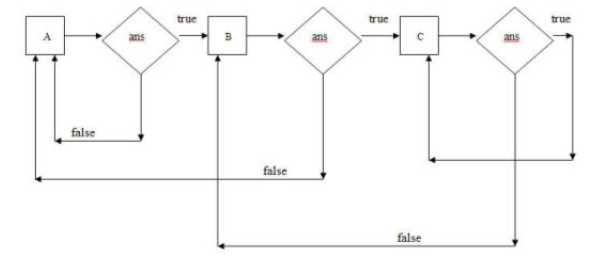
\includegraphics[width=\textwidth,height=\textheight,keepaspectratio]{PAT_adaptive_sequence}
\caption{Adaptive sequence of questions in PAT. (Source:\cite{PAT})}
\label{fig:PAT_adaptive_sequence}
\end{figure}

Figure \ref{fig:PAT_adaptive_sequence} shows the possible adaptive sequences. This algorithm is quite simplistic, every correct answer leads to a promotion to the next level of difficulty until no further promotions are possible. Likewise, every incorrect answer leads to a demotion to a lower level of difficulty until no further demotions are possible.\newline

At the end of the test, the system shows the student's total number of correct answers out of 30 and how well the student performed on each chapter. Also, PAT classifies the student into one of three programming skill levels based on their final score and a weighted score, where the difficulty of the questions answered correctly is considered. These results are available to both students and teachers so that they can be used to improve performance later on in the school year.\newline

We feel that the adaptive algorithm increases the difficulty of questions too quickly and doesn't take into account guessing or possible slip ups from students. This limitation can be circumvented by, for instance, requiring a number of correct answers at the current difficulty level before progressing to the next one.\newline

PAT only provides assessment at specific times throughout the school year and no opportunity for students to practice and self-assess in their own time. In addition, it isn't possible for teachers to upload their own questions to the system. The question bank remains static and contains 443 questions. Lastly, the authors of PAT admit that the statistical data available to students and teachers is fairly limited, and that improvements should be pursued in future work.

\section{Adaptive Self-Assessment Master}
Adaptive Self-Assessment Master (ASAM) is an extension to CourseMarker, which improves upon it by administering questions which are suited to the student's ability.

\section{SIETTE}
SIETTE\cite{SIETTE-small} (System of Intelligent Evaluation Using Tests for Tele-education) is a web based environment for generating and constructing adaptive tests. It has been used with great success in courses from the computer science engineering school, the telecommunication engineering school and the philosophy faculty, all at the University of Malaga, Spain.\newline

SIETTE is a vast system, and at the time of publication (2005) it contained information about $15000$ student test sessions, and the knowledge base contained 84 subjects, 1852 topics, 3820 question and 220 tests.\newline

SIETTE is designed to be used by both students and teachers. Teachers use the system to create tests, define the subject topics, the questions and their parameters. Students use the system to take the tests specified by the teachers. The tests can be used for self-assessment, where the correction is shown immediately after the student has answered. Hints and more extensive feedback are also available in this mode. Or, the tests can be used as exams, where the score counts towards the student's final grade. In this mode, hints and feedback aren't provided. It is important to note that tests have a fixed number of questions, thus, new tests must be created every time a student runs out of practice.\newline

As mentioned earlier, SIETTE constructs adaptive tests, therefore, when a student answers a question, his ability is re-estimated and the next question is selected accordingly. Implementation of this is done by using item response theory in the computerized adaptive testing framework.\newline

SIETTE uses the three-parameter logistic (3PL) model and measures the student's knowledge in terms of a discrete random variable $\theta$, which ranges from 0 to $K-1$, where $K$ is the number of discrete knowledge levels. When it comes to creating items, the guessing parameter $c$ is determined automatically, whereas the other two parameters must be entered by the teacher. The discrimination parameter ($a$) must be a number between $0.5$ and $1.5$. The difficulty parameter must be a natural number between 0 and $K-1$. A few years after the SIETTE paper was published, the authors added an item calibration tool because teacher estimates of item parameters are never very accurate.\newline

To estimate students' knowledge level, SIETTE uses the Bayesian estimation method (section \ref{subsec:IRT}) with a knowledge distribution per student, per topic. Also, SIETTE provides teachers with the option of choosing different item selection procedures for tests, such as random selection, difficulty-based selection and bayesian selection.

\begin{figure}[H]
\centering
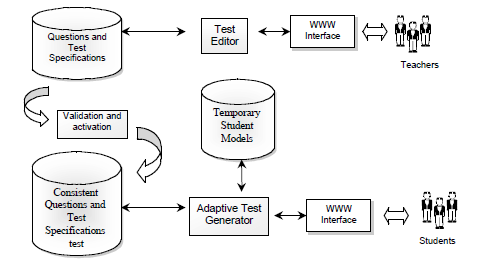
\includegraphics[width=\textwidth,height=\textheight,keepaspectratio]{siette-architecture}
\caption{SIETTE Architecture. (Source:\cite{SIETTE})}
\label{fig:siette-architecture}
\end{figure}

Figure \ref{fig:siette-architecture} gives on overview of the SIETTE architecture. The system is comprised of several components\cite{SIETTE-components}:
\begin{itemize}
\item The \textit{knowledge base}: where tests, topics and questions are stored. Some supported question types are true/false, multiple choice, multiple response and fill-in-the-gap. More interactive questions also exist, implemented as Java applets, where one has to color parts of a map, or move around objects so that they appear chronologically, for example.
\item The \textit{student model repository}: a collection of student models, where information about students' knowledge level estimation, which questions they answered, etc... is stored.
\item The \textit{student workspace}: a web interface where students take tests.
\item The \textit{test editor}: a tool where teachers can define tests, topics, questions.
\item The \textit{result analyzer}: a tool which presents graphical data about students' performance, knowledge estimation levels, etc...
\item The \textit{item calibration tool}: a module used to calibrate items by determining the item parameters (difficulty, discrimination and pseudo-chance).
\end{itemize}

SIETTE is a large and complex system, containing many useful features relevant to the area of web-education, and going through all of these wouldn't be possible. Since SIETTE has been used to such success in university courses we decide to inspire ourselves from this system, especially the implementation of the adaptive difficulty component. Details about the algorithms used in SIETTE, and hence jSCAPE, can be found in section 5.XX, with Java code to illustrate.

\section{Summary}
We have looked at some of the relevant work in the field of computer based education and assessment. We saw that SIETTE provided many of the features we set out to replicate in jSCAPE, therefore particular parts of our implementation will be inspired by SIETTE.

SIETTE the most complete system we have come across while doing research for this project.

Moreover, examining these existing solutions has given us insight into the most common features available in these types of systems.

We hope to have shown in this section that developing such systems is quite difficult since the depth of some features can be pushed quite far. Instead we decide to create a system which we deem as complete, having the main features present in the system but only the very basics of the feature, e.g. feedback is simple as opposed to complex feedback which would be more useful.

In the next chapter we present the system developed as part of this project: jSCAPE. 